% !TEX program = xelatex
\documentclass[aspectratio=169]{beamer}
\makeatletter
\def\@makefnmark{}
\makeatletter
\usepackage{amsthm,amsmath,amssymb,braket,fontspec,unicode-math,multimedia}
\usepackage[absolute,overlay]{textpos}
\usetheme[numbering=none]{focus}
\setbeamercolor{footnote}{fg=azure}
\setbeamerfont{footnote}{size=\tiny,series=\bfseries}
\setbeamerfont{alerted text}{series=\bfseries}
\setmathfont{Latin Modern Math}[range={frak,\bigcap,\bigcup,\checkmark}]

\usepackage[backend=bibtex,url=false,doi=false,maxcitenames=1, style=authoryear]{biblatex}
\bibliography{bib}
\AtBeginBibliography{\scriptsize}

\newcommand{\focus}[1]{\textcolor{red}{\bf{#1}}}
\AtBeginSection[]{}
\definecolor{red}{HTML}{CC0000}
\definecolor{lred}{HTML}{e24a33}
\definecolor{bgreen}{HTML}{006A4E}
\definecolor{azure}{HTML}{007fff}
\newcommand{\alertb}[1]{\color{azure}\alert{#1}}
\setbeamertemplate{bibliography item}[triangle]

\graphicspath{{./figures/}}

\title{{\LARGE URG Analysis of Electron in a Periodic Potential}\\ {\Large Role of the center of mass}}

\author{\textbf{Abhirup Mukherjee, Siddhartha Lal}}
\institute{\textbf{Emergent Phenomena in Quantum Matter} Group\\
Department of Physical Sciences, IISER Kolkata}

\date{July 21, 2023}
\begin{document}

\centering

\begin{frame}
\maketitle
\begin{textblock*}{0.13\textwidth}(13.5cm, 4.3cm)
	\centering

	
\includegraphics[width=\textwidth]{epqm_logo_mod.jpeg}\\
	\vspace*{\fill}
	
\includegraphics[width=\textwidth]{dps_logo.jpeg}
\end{textblock*}
\end{frame}

\section{The Big Picture}

\begin{frame}{The Big Picture}
\begin{itemize}[<+->]
	\item We reduce the problem to that of a \alert{particle placed on a ring} in a periodic potential and a gauge field (generated by the crystal momenta).\\[10pt]
	\item By applying the URG to this problem, we show the \alert{emergence of bands}.\\[10pt]
	\item We then elucidate certain important physical ideas like the role of the particle on a circle problem as the \alert{center of mass} of the system and the connection of the gauge field to Bloch’s theorem.\\[10pt]
	\item We demonstrate that the metal-insulator transition observed upon tuning the chemical potential occurs through the change of a \alert{topological number}.\\[10pt]
	\item We conclude by connecting this problem to that of the \alert{IQHE}.
\end{itemize}
\end{frame}

\section{The Problem of a Particle in a Periodic Potential}

\begin{frame}{The Problem of a Particle in a Periodic Potential (PPP)}
	\[\mathcal{H} = \int_{-\infty}^{\infty}\mathrm{dx}~c^\dagger(x)\left[\hat p^2/2m + V(x)\right]c(x),\quad V(x+a) = V(x)\]
	\only<1>{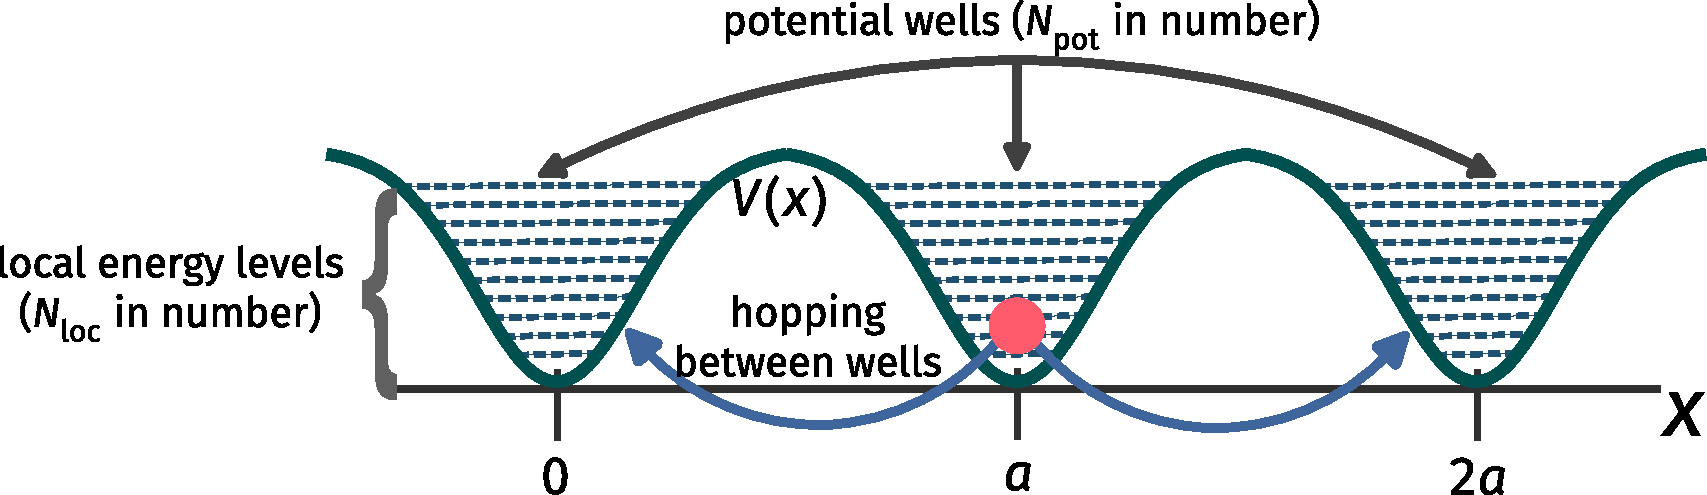
\includegraphics[width=0.9\textwidth]{potential.pdf}}
	\only<2>{
	\begin{minipage}{0.4\textwidth}
	Potential only connects momentum states separated by a reciprocal lattice vector.
	\[\braket{k+q | V | k} = \delta_{q,G} V(G)\]
	Leads to conserved \\ \alert{crystal momenta}: \(\left\{ k_j < G \right\} \)
	\end{minipage}
	\hspace*{\fill}
	\begin{minipage}{0.5\textwidth}
	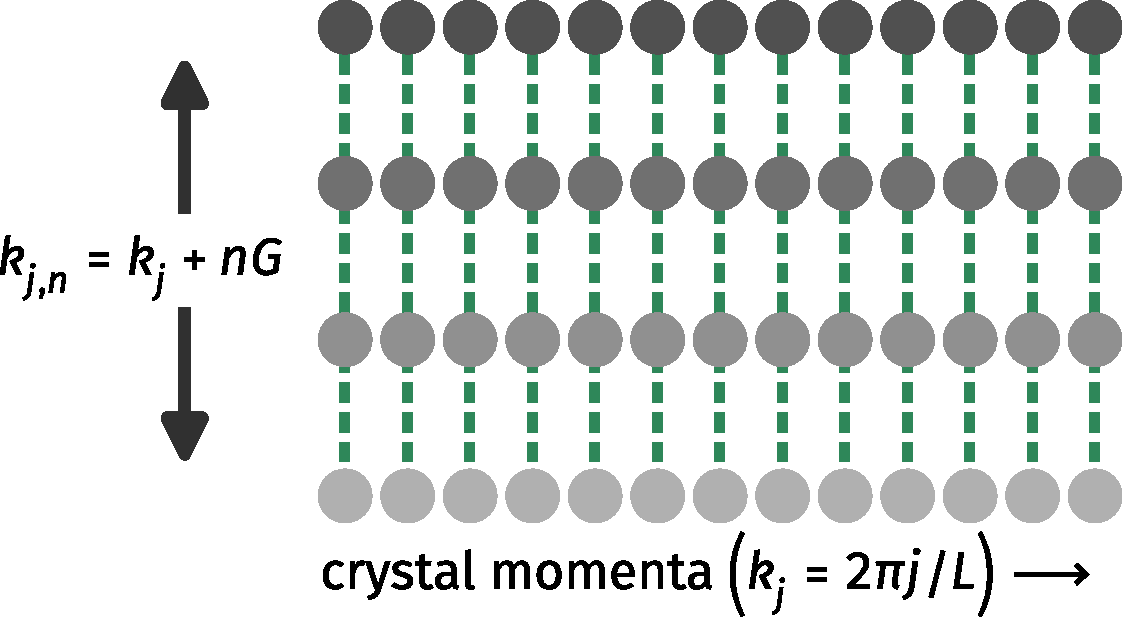
\includegraphics[width=\textwidth]{momentum_states.pdf}
	\end{minipage}
	}
\end{frame}

\section{The PPP as a Particle on a Circle}
\subsection{~}

\begin{frame}{The PPP as a Particle on a Circle}
	The conserved crystal momenta leads to a block-diagonal form of the Hamiltonian.
	\[\mathcal{H} = \sum_k \mathcal{H}(k), \quad \mathcal{H}(k) \sim \left( -i\hbar\frac{\partial}{\partial x^\prime} + \hbar k\right)^2 + V(x^\prime)\]

	\vspace*{\fill}
	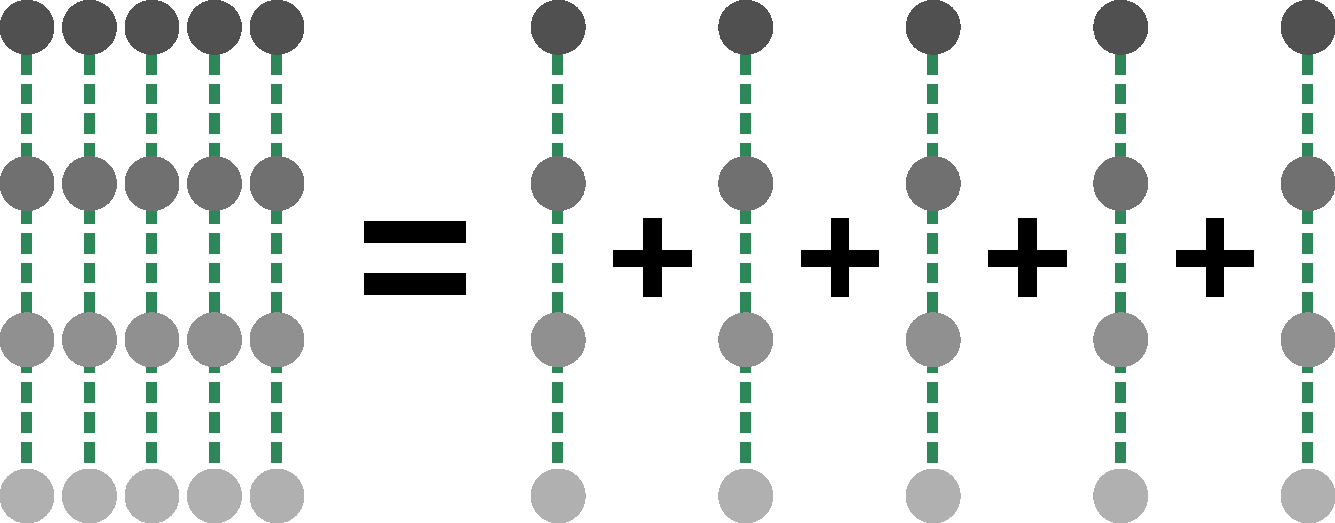
\includegraphics[width=0.5\textwidth]{decomposition.pdf}
\end{frame}

\begin{frame}{The PPP as a Particle on a Circle}
	Define dimensionless position and momentum.
	\[\mathcal{H}(k) = \frac{\hbar^2}{2ma^2}\left(\hat Q + \Phi/2\pi\right)^2 + U(\theta)\]

	\vspace*{\fill}
	Hamiltonian is that of a \alert{particle on a circle}. Flux is \(\Phi = ka\).

	\vspace*{\fill}
	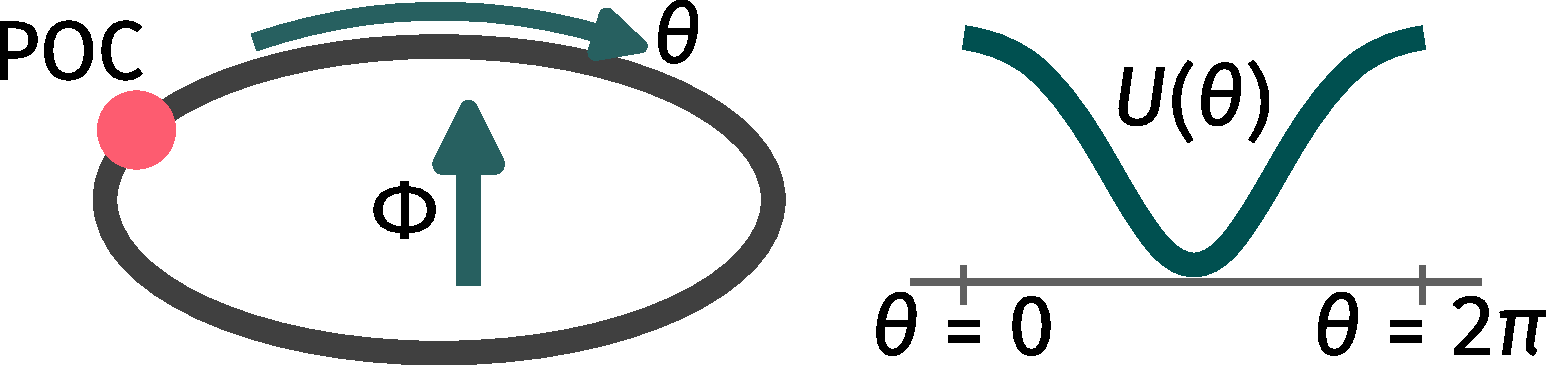
\includegraphics[width=0.6\textwidth]{POC.pdf}
\end{frame}

\section{URG Analysis of the POC}
\subsection{~}

\begin{frame}{URG Analysis of the PAC}
	\alert{Resolve fluctuations} in angular momentum states by applying unitary transformations.
	\[\Delta \mathcal{U}_{ij}^{(l)}(\omega) = \frac{\mathcal{U}_{il}\mathcal{U}_{lj}}{\omega - \varepsilon(Q_l + \Phi/2\pi)},\quad U_{ij} = U(Q_i - Q_j)\]
	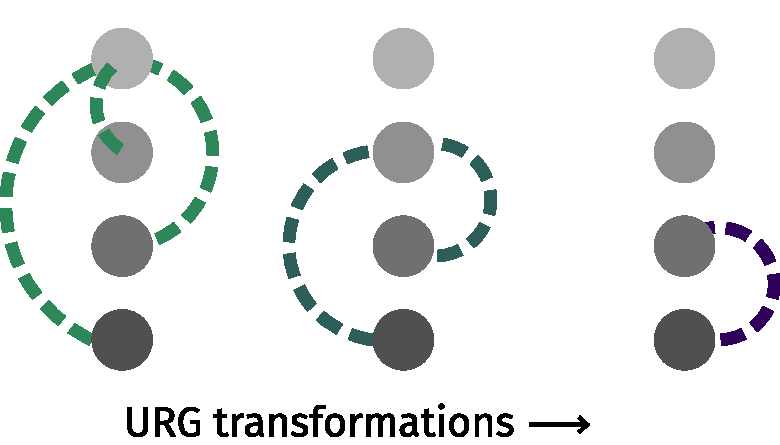
\includegraphics[width=0.4\textwidth]{URG_poc.pdf}
\end{frame}

\begin{frame}{Appearance of band gaps}
\only<1>{
	\alert{Effective Hamiltonian} for the final two states:
	\begin{minipage}{0.7\textwidth}
	\[H_{01}^* = \varepsilon^*(Q_0)\ket{Q_0}\bra{Q_0} + \varepsilon^{*}(Q_1)\ket{Q_1}\bra{Q_1} + \left(\mathcal{U}_{01}^{*}\ket{Q_1}\bra{Q_0} + \text{h.c.}\right)\]
	Diagonalise the final Hamiltonian: \(E_\pm = \varepsilon^* \pm |\mathcal{U}_{01}^*|\)\\
	\begin{minipage}{0.5\textwidth}
	Gives the \alert{shifts in energies}: 
	\end{minipage}
	\begin{minipage}{0.45\textwidth}
	\[\Delta \varepsilon^* \simeq \frac{|\mathcal{U}_{01}^*|^2}{\varepsilon^* \pm |\mathcal{U}_{01}^*| - \varepsilon^*} \simeq \pm |\mathcal{U}_{01}^*|\]
	\end{minipage}
	\end{minipage}
	\hspace*{\fill}
	\begin{minipage}{0.2\textwidth}
	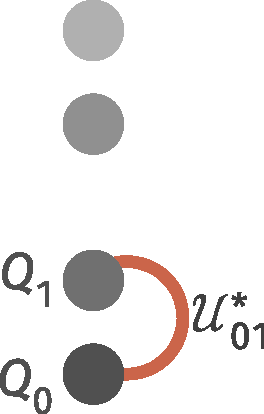
\includegraphics[width=0.7\textwidth]{effham10.pdf}
	\end{minipage}
}
\only<2>{
	Allow the flux \(\Phi\) to vary:
	\[\varepsilon^*(\Phi) - |\mathcal{U}^*_{01}|; \Phi = ak\]
	Creates the \alert{first band}!

	\vspace*{\fill}
	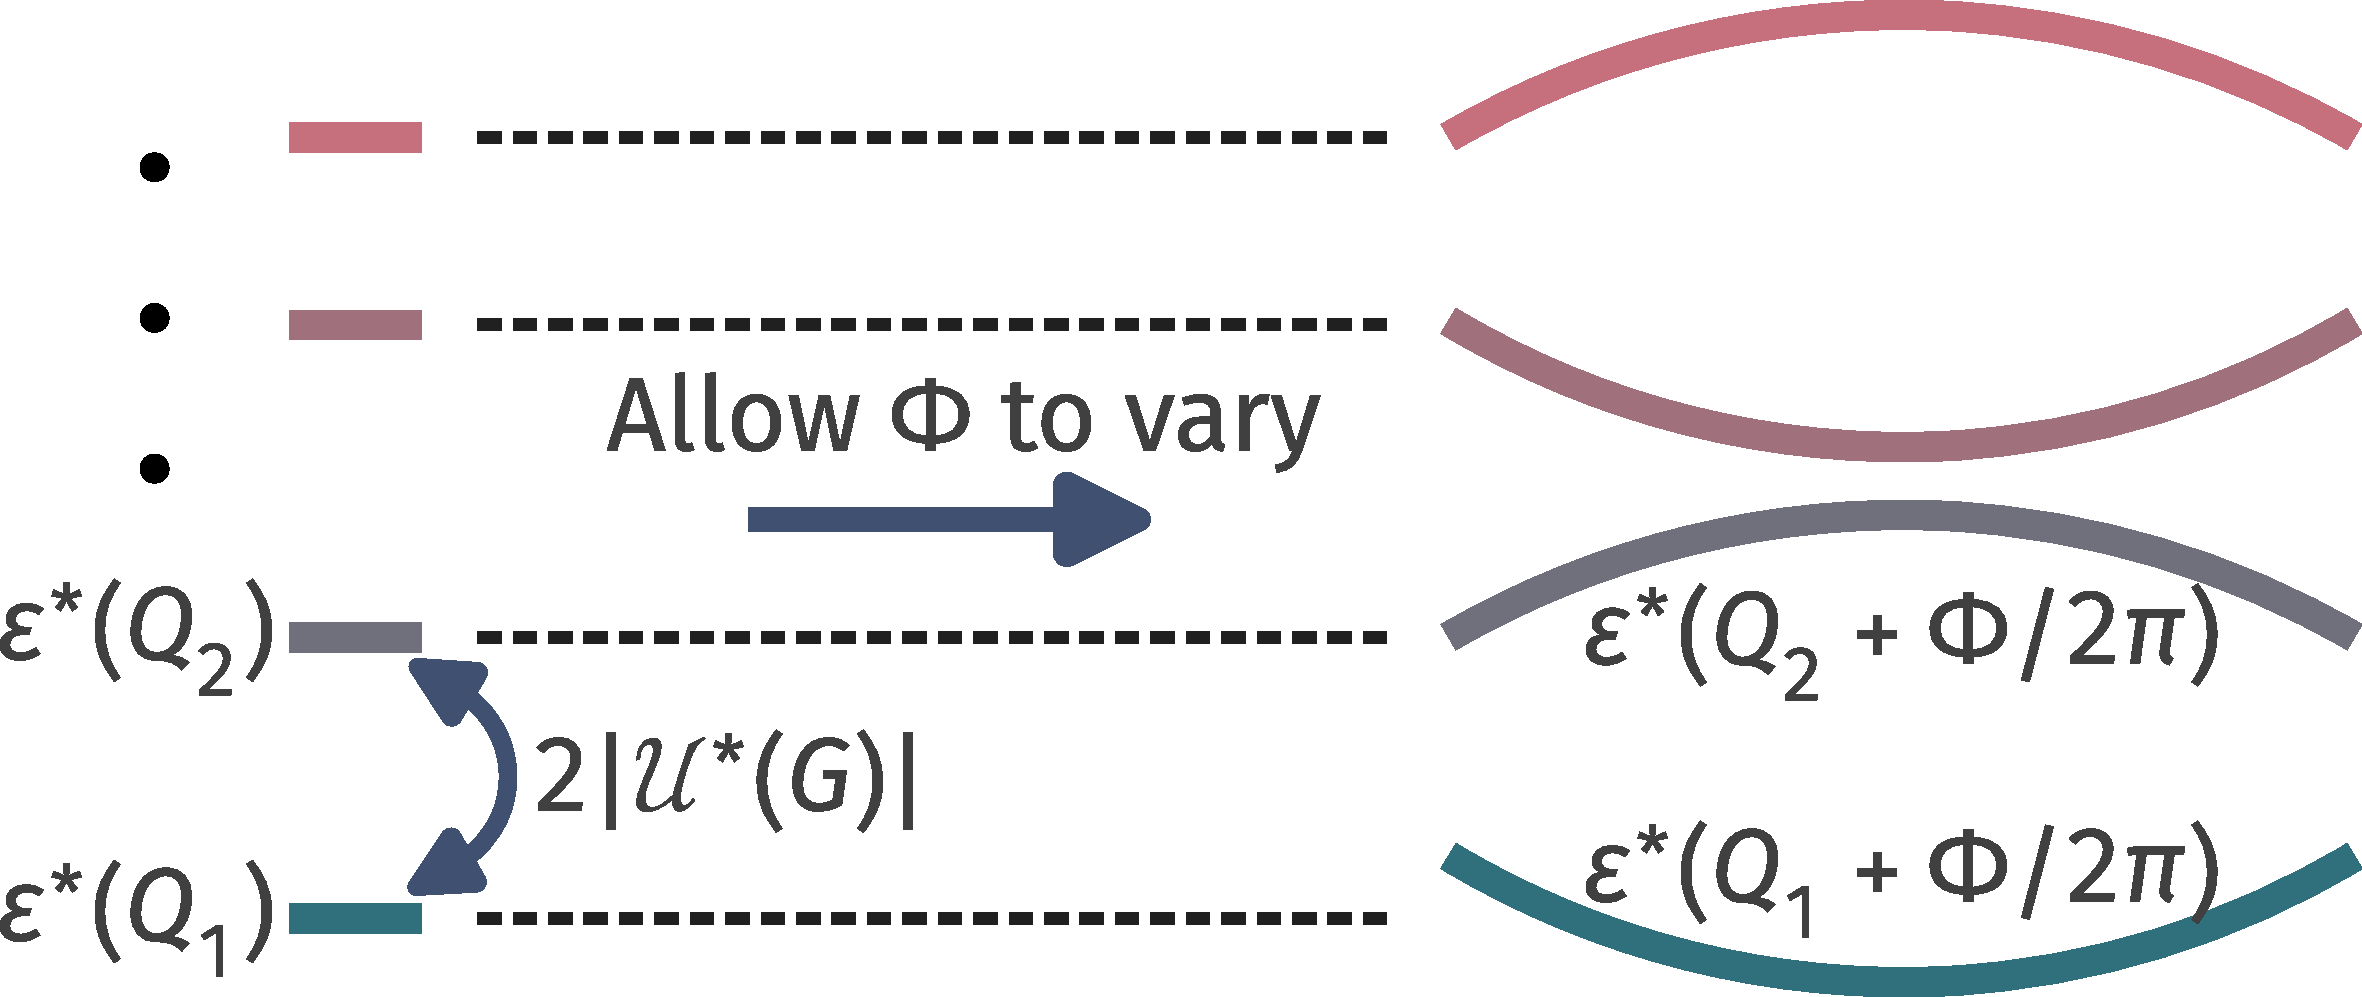
\includegraphics[width=0.7\textwidth]{URGSpectrum.pdf}
}

\end{frame}

\begin{frame}{Dispersion for the lowest band}
	\only<1>{
	Fixed point Hamiltonian for the lowest state is of the form:
	\[\varepsilon^*(Q_0)\ket{Q_0}\bra{Q_0}\]

	\vspace*{\fill}

	\begin{minipage}{0.6\textwidth}
	Involves only longest-range hopping:
	\[ \frac{1}{2}\varepsilon^{*}(2\pi)\left( \hat n(0) + \hat n(2\pi) \right) + \frac{1}{2}\varepsilon^{*}(2\pi)\left(c^\dagger(0)c(2\pi) + \text{h.c.}\right)\]
	\end{minipage}
	\hspace*{\fill}
	\begin{minipage}{0.3\textwidth}
	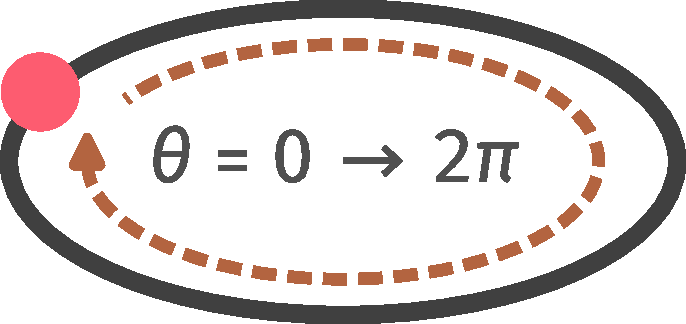
\includegraphics[width=\textwidth]{longhopping.pdf}
	\end{minipage}

	\vspace*{\fill}
	\begin{minipage}{0.6\textwidth}
	Can be transformed back to real space: \(\theta \to x^\prime\)
	\[ \frac{1}{2}\varepsilon^{*}(2\pi)\left( \hat n(0) + \hat n(a) \right) + \frac{1}{2}\varepsilon^{*}(a)\left(c^\dagger(0)c(a) + \text{h.c.}\right)\]
	\end{minipage}
	\hspace*{\fill}
	\begin{minipage}{0.3\textwidth}
	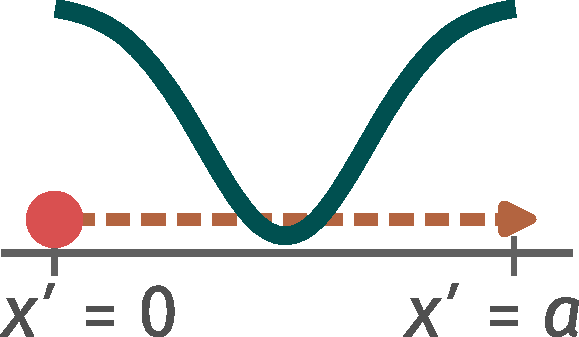
\includegraphics[width=\textwidth]{longhoppingreal.pdf}
	\end{minipage}
}
\only<2>{

	\begin{minipage}{0.3\textwidth}
	Reintroduce the flux.\\[10pt]
	Equivalent to translating over all lattice sites.\\[10pt]
	\end{minipage}
	\hspace*{\fill}
	\begin{minipage}{0.6\textwidth}
	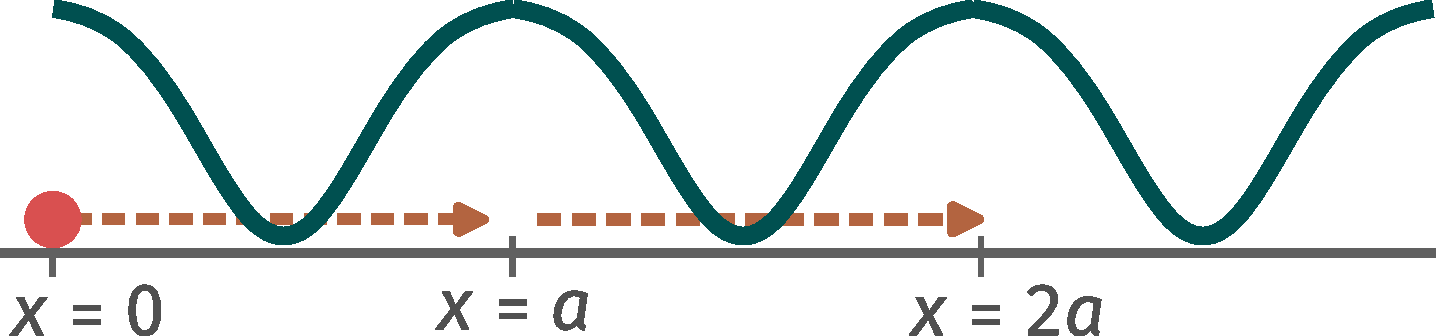
\includegraphics[width=\textwidth]{tightbinding.pdf}
	\end{minipage}

	\vspace*{\fill}
	Leads to a tight-binding model!
	\[H_{TB} = \varepsilon^{*}(2\pi)\sum_{j=0}^{N_\text{well}-1}\hat n(ja) + \frac{1}{2}\varepsilon^{*}(a)\sum_{j=0}^{N_\text{well}-1}\left(c^\dagger(ja)c((j+1)a) + \text{h.c.}\right)\]
}
\end{frame}

\section{Insights on the crystal momentum, role of the POC, and Bloch’s theorem}
\subsection{~}

\begin{frame}{The crystal momentum as a magnetic flux}
\begin{itemize}
	\item Crystal momentum acts like a gauge field for the POC\\[10pt]
	\item Leads to twisted boundary conditions for the POC\\[10pt]
	\item Topological in nature (akin to a \(\theta-\)term in the action)
\end{itemize}
\end{frame}

\begin{frame}{Berry phase and Bloch’s theorem}
\begin{minipage}{0.5\textwidth}
Bloch's theorem for periodic potential:
\[\psi_k(x + ma) = e^{-ikam}\psi_k(x)\]
\end{minipage}
\hspace*{\fill}
\begin{minipage}{0.45\textwidth}
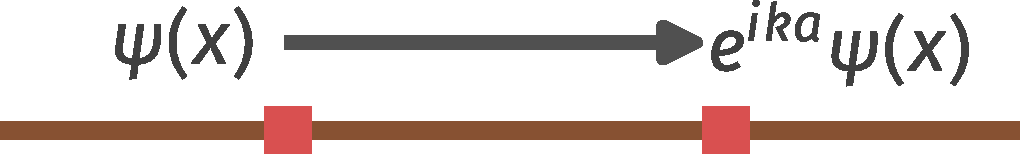
\includegraphics[width=\textwidth]{blochtheorem.pdf}
\end{minipage}

\vspace*{\fill}
\begin{minipage}{0.5\textwidth}
Equivalent to the Berry phase acquired in the presence of a flux!\\[10pt]
\end{minipage}
\hspace*{\fill}
\begin{minipage}{0.45\textwidth}
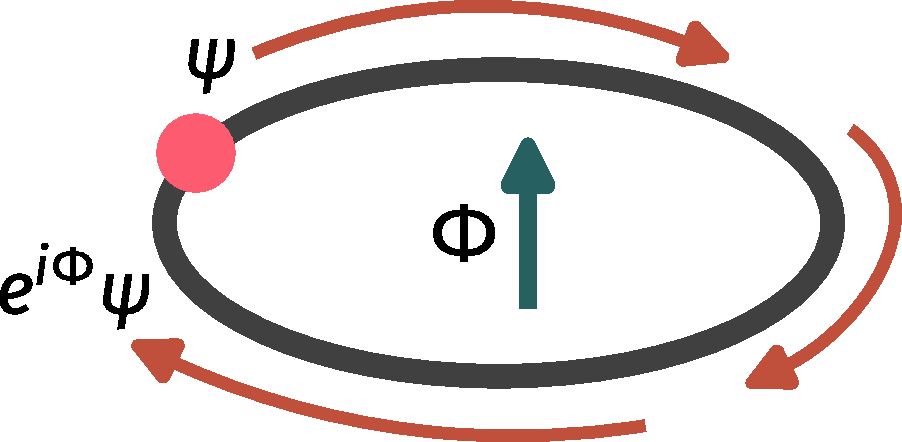
\includegraphics[width=\textwidth]{berryphase.pdf}
\end{minipage}

\vspace*{\fill}
Crystal momentum therefore acts as a Berry phase, sensitive to the topology of PBC!
\end{frame}

\begin{frame}{The POC as a centre of mass}
The PPP problem can be mapped to the problem \\
of a single well but in a variable flux.

\vspace*{\fill}
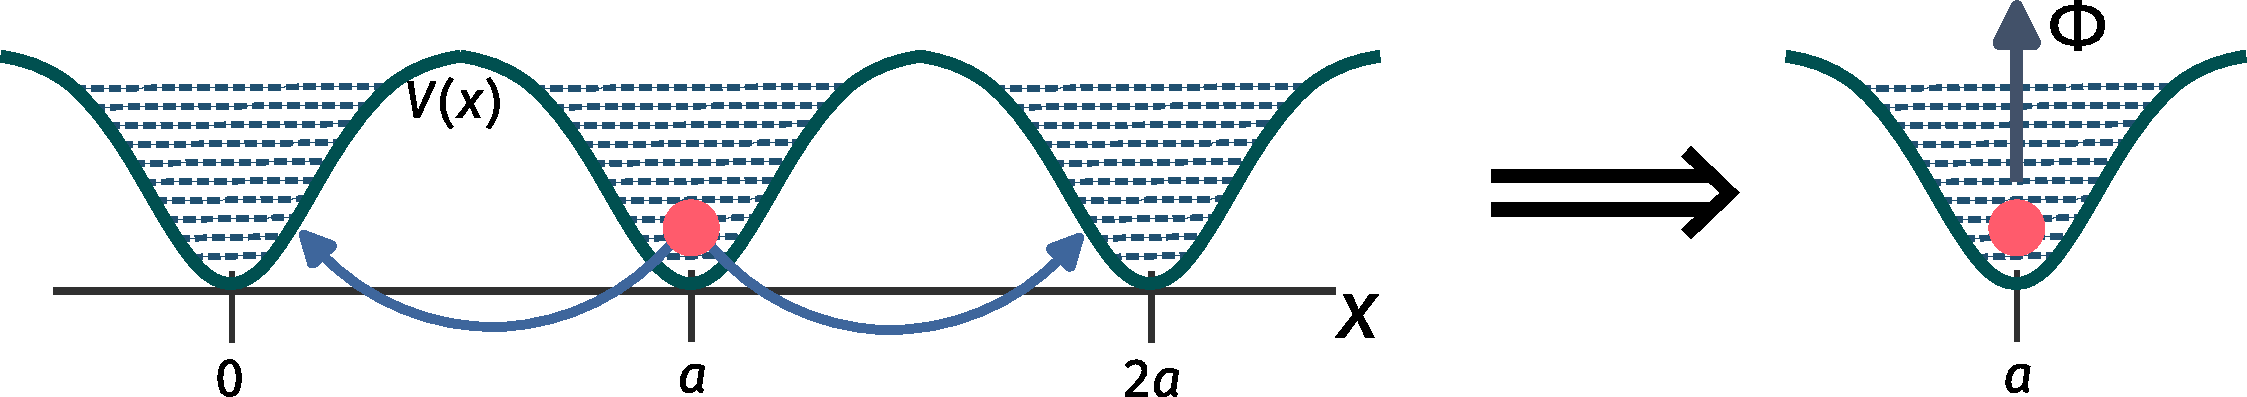
\includegraphics[width=\textwidth]{centerofmass.pdf}

\vspace*{\fill}
The POC can be thought of as the \alert{center of mass} degree of freedom.
\end{frame}

\section{Metal-insulator transition}

\begin{frame}{Metal-insulator transition upon tuning chemical potential}
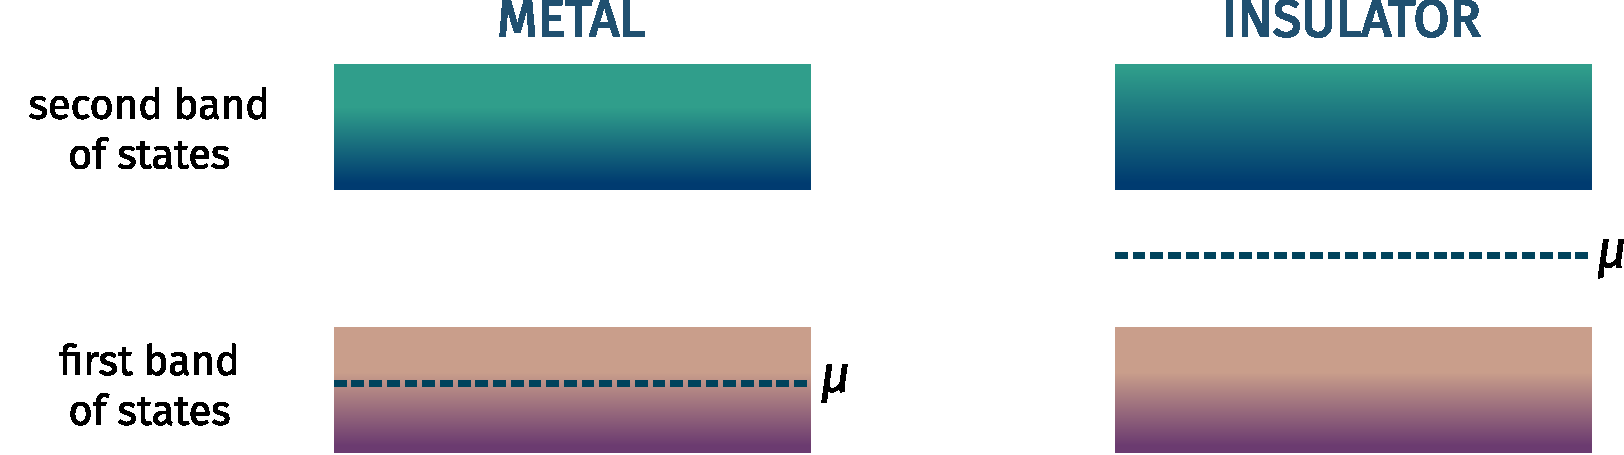
\includegraphics[width=\textwidth]{transition.pdf}

\vspace*{\fill}
\hspace*{\fill}~possibility of spectral flow~\hspace*{\fill}~no possibility of spectral flow
\end{frame}

\begin{frame}{Topological nature of the transition}
\only<1>{
Greens function has poles at the energy eigenvalues:
\(G(z) = \sum \left(z - E_i(\Phi_m)\right)^{-1}\)

\vspace*{\fill}
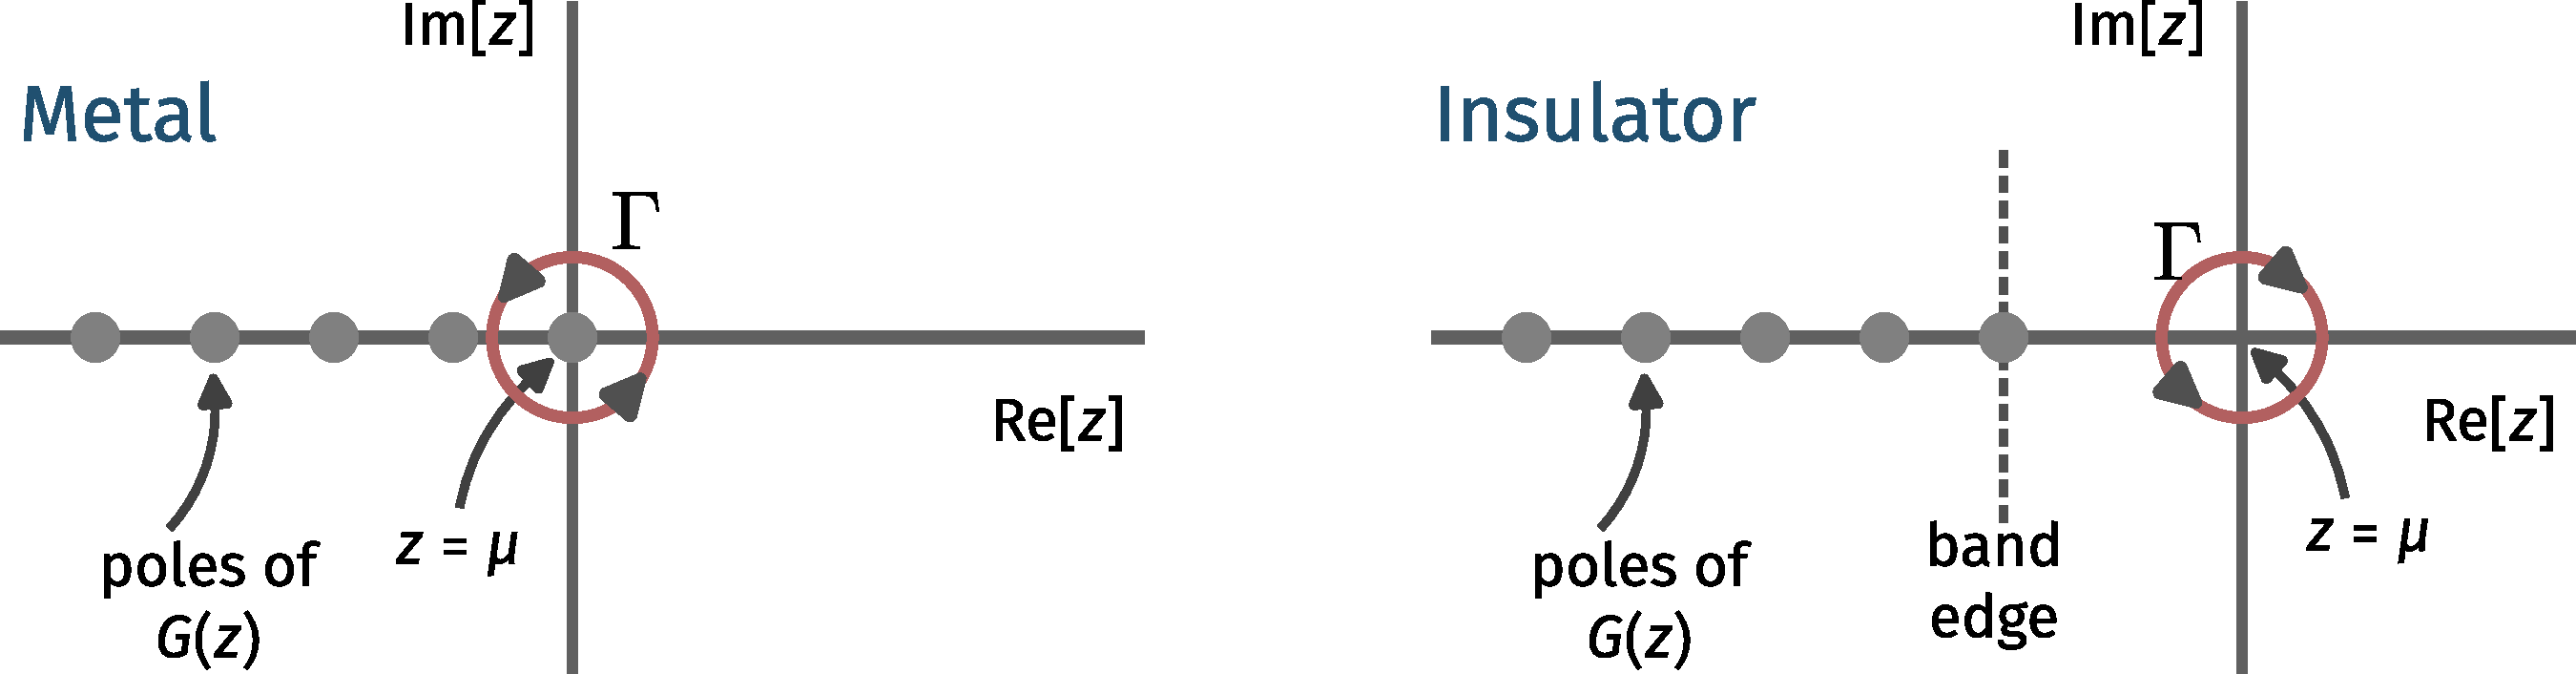
\includegraphics[width=\textwidth]{contour.pdf}

\vspace*{\fill}
\begin{minipage}{0.5\textwidth}
Fermi level occupancy can be detected through presence of pole:
\end{minipage}
\hspace*{\fill}
\begin{minipage}{0.4\textwidth}
	\[n_\text{FL} = \frac{1}{2\pi i}f_\text{FD}(\mu) \oint_\Gamma \mathrm{dz}~ \text{Tr}\left[\mathbf{G}(z)\right]\]
\end{minipage}
}
\only<2>{
Fermi level occupancy can be expressed as a winding number:
\[n_\text{FL} = \frac{1}{2\pi i} \oint_\Gamma \mathrm{dz}~ \frac{d}{dz}\ln \text{Det}\left[\mathbf{G}^{-1}\right] = \text{some integer}\]

\vspace*{\fill}
Counts the number of times \(\ln \text{Det}\left[\mathbf{G}^{-1}\right](\Gamma)\) winds around the origin.

\vspace*{\fill}
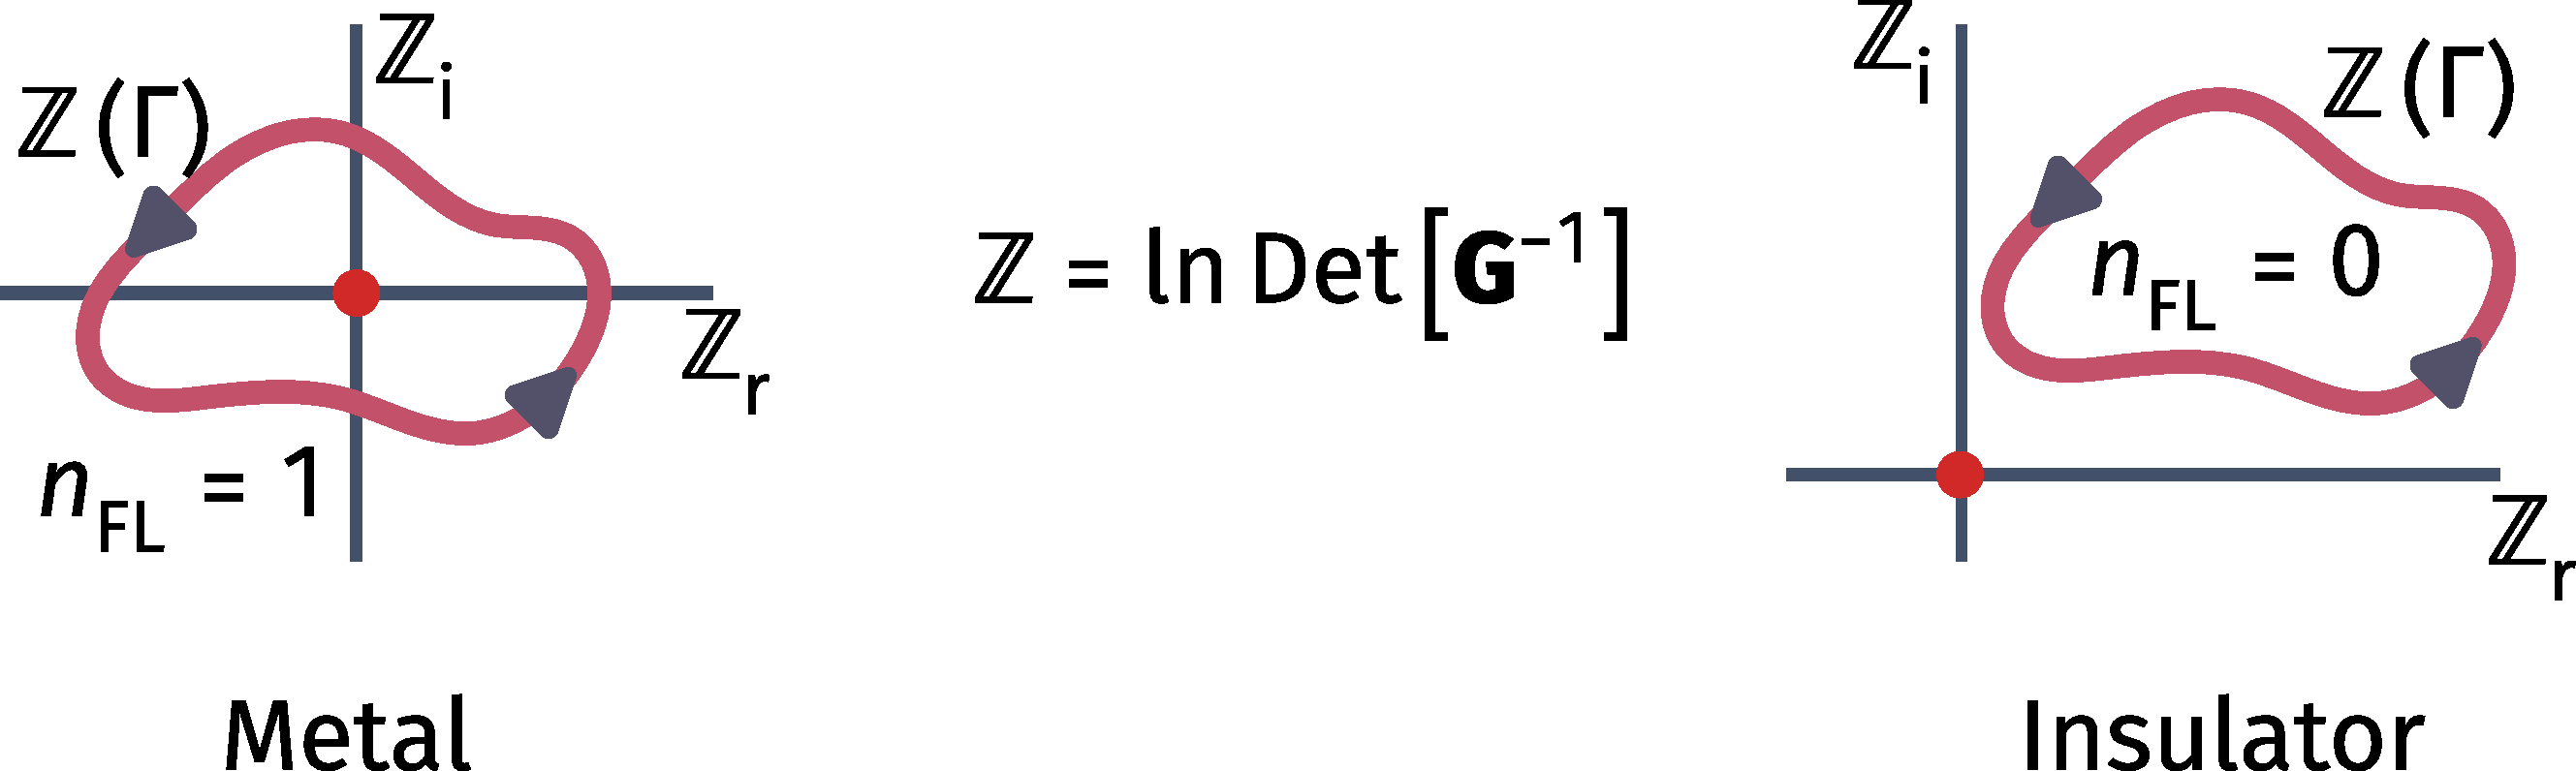
\includegraphics[width=0.8\textwidth]{winding.pdf}
}

\end{frame}
\begin{frame}[c]{}
	\LARGE{THANK YOU.}
\end{frame}

\end{document}
